%%%%%%%% ICML/ICCV 2021 EXAMPLE LATEX SUBMISSION FILE %%%%%%%%%%%%%%%%%

\documentclass[10pt,onecolumn,letterpaper]{article} % comment out for ICCV style paper
%\documentclass[onecolumn]{article} % comment out for NeurIPS style paper

\usepackage{etex}
\usepackage{todonotes}

% MN: to create different versions
%\usepackage[icml_submission]{optional}
%\usepackage[icml_accepted]{optional}
%\usepackage[for_gig]{optional}
\usepackage[iccv_submission]{optional}

\opt{iccv_submission}{
  \usepackage{iccv_supplementary}
  \usepackage{times}
  \usepackage{epsfig}
  \usepackage{graphicx}
  \usepackage{amsmath}
  \usepackage{amssymb}
  \usepackage{listings} 
  % Include other packages here, before hyperref.
  
  % If you comment hyperref and then uncomment it, you should delete
  % egpaper.aux before re-running latex.  (Or just hit 'q' on the first latex
  % run, let it finish, and you should be clear).
  \usepackage[pagebackref=true,breaklinks=true,letterpaper=true,colorlinks,bookmarks=false]{hyperref}
  
  \iccvfinalcopy % *** Uncomment this line for the final submission
  
  \def\iccvPaperID{10828} % *** Enter the ICCV Paper ID here
  \def\httilde{\mbox{\tt\raisebox{-.5ex}{\symbol{126}}}}

  % Pages are numbered in submission mode, and unnumbered in camera-ready
  \ificcvfinal\pagestyle{empty}\fi


}

\opt{icml_submission,for_gig}{
  \usepackage{graphicx}
  \usepackage{amsmath}
  \usepackage{amssymb}
  \usepackage[colorlinks=true,linkcolor=blue,citecolor=blue]{hyperref}
  \usepackage[table]{xcolor}
}



% Recommended, but optional, packages for figures and better typesetting:
\usepackage{microtype}
\usepackage{subfigure}
\usepackage{booktabs} % for professional tables

\usepackage{enumitem}

\usepackage{amsfonts}

\usepackage{tikz}

\usetikzlibrary{arrows.meta, % if the figure contains arrow-tips
                bending,     % arrow tips on arcs are "bent," i.e., deformed a bit
                patterns     % if the figure contains pattern fills
               }

\usetikzlibrary{spy}
\usetikzlibrary{arrows,shapes,automata,backgrounds,petri,positioning}
\usetikzlibrary{decorations.pathmorphing}
\usetikzlibrary{decorations.shapes}
\usetikzlibrary{decorations.text}
\usetikzlibrary{decorations.fractals}
\usetikzlibrary{decorations.footprints}
\usetikzlibrary{shadows}


\renewcommand\floatpagefraction{.99}
\renewcommand\topfraction{.99}
\renewcommand\bottomfraction{.99}
\renewcommand\textfraction{.01}   
\setcounter{totalnumber}{50}
\setcounter{topnumber}{50}
\setcounter{bottomnumber}{50}

%\setlength{\textfloatsep}{0.25\baselineskip plus 0.2\baselineskip minus 0.5\baselineskip}

\setlength{\textfloatsep}{1.25\baselineskip plus 0.2\baselineskip minus 0.5\baselineskip}

\DeclareMathOperator{\id}{Id}
\newcommand{\fxpsi}{\Phi_{\theta}^{BA}}
\newcommand{\fxvarphi}{\Phi_{\theta}^{AB}}
\newcommand{\fxpsivarepsilon}{\Phi_{\theta \varepsilon}^{BA}}
\newcommand{\fxvarphivarepsilon}{\Phi_{\theta \varepsilon}^{AB}}
\graphicspath{{figs/}}

\newcommand{\mn}[1]{{\color{blue}{#1}}}
\newcommand{\mnl}[1]{{\color{red}{$\leftarrow$~#1}}}
\newcommand{\mnr}[1]{{\color{red}{#1~$\rightarrow$}}}
\newcommand{\zp}[1]{{\color{blue}{#1}}}
\newcommand{\fx}[1]{{\color{magenta}{#1}}}

% hyperref makes hyperlinks in the resulting PDF.
% If your build breaks (sometimes temporarily if a hyperlink spans a page)
% please comment out the following usepackage line and replace
% \usepackage{icml2021} with \usepackage[nohyperref]{icml2021} above.
%\usepackage{hyperref}

% Attempt to make hyperref and algorithmic work together better:
\newcommand{\theHalgorithm}{\arabic{algorithm}}

\opt{icml_submission}{
% Use the following line for the initial blind version submitted for review:
\usepackage{icml2021}

\usepackage{setspace}
\usepackage[labelfont={bf,small},font={small,stretch=1.1}]{caption}
%\usepackage{subcaption}

\usepackage[colorinlistoftodos,prependcaption,textsize=tiny]{todonotes}
}

\opt{icml_accepted}{
% If accepted, instead use the following line for the camera-ready submission:
  \usepackage[accepted]{icml2021}
}

\opt{for_gig}{
  \usepackage[accepted]{icml2021_unpublished_draft}
  \usepackage[colorinlistoftodos,prependcaption,textsize=tiny,disable]{todonotes}
  % disable todos
  %\usepackage[colorinlistoftodos,prependcaption,textsize=tiny,disable]{todonotes}
}
\pagenumbering{roman}
\begin{document}

\sloppy

\opt{iccv_submission}{
  %%%%%%%%% TITLE
\title{ICON: Supplementary Material}

\author{Hastings Greer\\
  Department of Computer Science\\
UNC Chapel Hill, USA\\
{\tt\small tgreer@cs.unc.edu}
% For a paper whose authors are all at the same institution,
% omit the following lines up until the closing ``}''.
% Additional authors and addresses can be added with ``\and'',
% just like the second author.
% To save space, use either the email address or home page, not both
\and
Roland Kwitt\\
Department of Computer Science\\
University of Salzburg, Austria\\
{\tt\small Roland.Kwitt@sbg.ac.at}
\and
Fran\c{c}ois-Xavier Vialard\\
LIGM, Universit\'e Gustave Eiffel, France\\
{\tt\small francois-xavier.vialard@u-pem.fr}
\and
Marc Niethammer\\
 Department of Computer Science\\
UNC Chapel Hill, USA\\
{\tt\small mn@cs.unc.edu}
}

\maketitle
% Remove page # from the first page of camera-ready.
\ificcvfinal\thispagestyle{empty}\fi
}
\thispagestyle{plain}
\pagestyle{plain}

\opt{for_gig,icml_submission}{

% The \icmltitle you define below is probably too long as a header.
% Therefore, a short form for the running title is supplied here:
%\icmltitlerunning{Inverse Consistency is Almost All You Need}
\icmltitlerunning{Learning Regular Maps Through Inverse Consistency}
  
\onecolumn[
%\icmltitle{Inverse Consistency is All You Need \\ -- for Image Registration}
\icmltitle{Learning Regular Maps Through Inverse Consistency}

\icmlsetsymbol{equal}{*}

\begin{icmlauthorlist}
\icmlauthor{Hastings Greer}{unc}
\icmlauthor{Roland Kwitt}{salzburg}
\icmlauthor{Fran\c{c}ois Xavier-Vialard}{upem}
\icmlauthor{Marc Niethammer}{unc}
\end{icmlauthorlist}

\icmlaffiliation{unc}{Department of Computer Science, University of North Carolina at Chapel Hill, USA}
\icmlaffiliation{salzburg}{Department of Computer Science, University of Salzburg, Austria}
\icmlaffiliation{upem}{LIGM, Universit\'e Gustave Eiffel, France}

\icmlcorrespondingauthor{Hastings Greer}{tgreer@cs.unc.edu}

\icmlkeywords{Deep Learning, Image Registration, Inverse Consistency}

\vskip 0.3in
]

%\printAffiliationsAndNotice{}  % leave blank if no need to mention equal contribution
\printAffiliationsAndNotice{\icmlEqualContribution} % otherwise use the standard text.
}

\sloppy

%\onecolumn
\section*{Introduction}
We cover these topics in the supplementary material that did not fit into the main manuscript:
\begin{itemize}
\item We retrace the proof of the $H^1$ regularizing property of approximate inverse consistency in greater detail.
\item We specify all details of the neural network architectures used in the manuscript's experiments, including number of features, number of layers, training proceedure, etc.
\end{itemize}

\section{Detailed proof of the regularizing effect of inverse consistency}

This section details our derivation for the smoothness properties emerging from approximate inverse consistency. 

%\subsection{Smoothness via approximate inverse consistency} 

%We now give arguments for the regularizing properties of approximate inverse consistency in the context of pairwise image registration.
Denote by $\fxvarphi(x)$ the output map of a network for images $(I^A,I^B)$ and by $\fxpsi(x)$ the output map between $(I^B,I^A)$
%\todo{FX, I put this back in. There was somehow something missing in the text.}.
%FX: ok
%In practice, this map is only defined at grid points, but we extend it to the full domain by interpolation. %However, our arguments apply quite independently of how the maps are actually computed.
%Inverse consistency by itself does not prevent discontinuous solutions, we propose to use approximate inverse consistency to favor $C^0$ solutions. 
%We now show that once diffeomorphic solutions have been favored, an implicit $H^1$ regularization emerges from the introduction of the noise.
Recall that we add two independent spatial white noises $n_1(x),~n_2(x)\in\mathbb{R}^N$ ($x \in [0,1]^N$ with $N = 2$ or $N = 3$ the dimension of the image)
%$n_1(i,x),n_2(i,x)$
%($i = 1,\ldots,N$; $x \in [0,1]^N$ with $N = 2$ or $N = 3$ the dimension of the image)
of variance $1$ for each spatial location to the two output maps and define $\fxvarphivarepsilon(x) := \fxvarphi(x) + \varepsilon n_1(\fxvarphi(x))$ and $\fxpsivarepsilon(x) := \fxpsi(x) + \varepsilon n_2(\fxpsi(x))$ with $\varepsilon$ a positive parameter.
We consider the following loss
\begin{multline}\label{EqLossSymmetric2}
    \mathcal{L} =\lambda \left( \| \fxvarphivarepsilon \circ \fxpsivarepsilon - \operatorname{Id} \|^2_2 + \| \fxpsivarepsilon \circ \fxvarphivarepsilon - \operatorname{Id} \|^2_2 \right) + \| I^A \circ \fxvarphi - I^B \|^2_2 + \| I^B \circ \fxpsi  - I^A \|^2_2\,.
\end{multline}
%where $\| \cdot \|^2$ is the sum-of-squares loss.
%Importantly, remark that there are multiple maps that can lead to the same $I^A \circ \fxvarphi$ and $I^B \circ \fxpsi$. Therefore, among all these maps,  the minimization of the loss $\mathcal{L}$ drives the maps towards those minimizing the first two terms.
%When minimizing the loss $\mathcal{L}$, it is clear that fixing
%
%\todo{Why should we fix this? Is this not a joint optimization problem in $\theta$?} 
% FX: in fact, this is the indeterminacy of the transformation on the regions of the flat areas of the images that I want to refer to. Multiple deformations can lead to the same result
%
%
%$I^A \circ \fxvarphi$ and $I^B \circ \fxpsi$, one is left with the minimization of the two first terms.
%We make the following assumption:
%\par
%\textbf{Assumption: }
%\emph{The minimization of the two first terms can be driven to a small value of the order of the noise.}
%\par
%Our experiments in Sec.~\ref{section:experiments} will verify this assumption.
%\todo{I removed the sentence afterwards. Not sure if you think it was essential. THe one that starts with ``Note however''.}
% FX: I am ok to remove it.
%
%Note however, that one might have to train the network for a long time in order to get the matching part of the loss very stable so that the gradient descent only optimizes on the first part of the loss.
%The network acts transitively on the dataset via smooth invertible maps. I.e., for any given image pair $(I^A,I^B)$ of the training dataset, there exist outputs of the network which are inverse consistent and smooth. As a consequence, when considering only a pair of images $(I^A,I^B)$ the last two terms of the loss \eqref{EqLossSymmetric} can be made zero by the network, therefore \emph{the overall error after training is of the order of the energy of the noise}, if a global minima is reached. 
Throughout this section, we give the details of the expansion in $\varepsilon$ of the loss, thus we use the standard notations $o$ and $O$ w.r.t $\varepsilon \rightarrow 0$.
We focus on the first two terms (that we denote by $\lambda \mathcal{L}_{\text{inv}}$) since the regularizing property comes from the inverse consistency.
We expand one of the first two terms  of \eqref{EqLossSymmetric2} since by symmetry the other is similar. If the noise is bounded (or with high probability in the case of Gaussian noise), we have
\begin{equation}
  \| \fxvarphivarepsilon \circ \fxpsivarepsilon - \operatorname{Id} \|^2_2 =   \| \fxvarphi \circ \fxpsi + \varepsilon n_1(\fxvarphi \circ \fxpsi)  + d\fxvarphivarepsilon(\varepsilon n_2(\fxpsi)) - \operatorname{Id}\|^2_2 + o(\varepsilon^2)\,,
\end{equation}
where $d\Phi$ denotes the Jacobian of $\Phi$. By developing the squares and taking expectation, we get 
\begin{multline}\label{EqExpectation}
    \mathbb{E}[\| \fxvarphivarepsilon \circ \fxpsivarepsilon - \operatorname{Id} \|^2_2] = \| \fxvarphi \circ \fxpsi - \operatorname{Id} \|^2_2 + \varepsilon^2 \mathbb{E}[\|n_1\circ(\fxvarphivarepsilon \circ \fxpsivarepsilon)\|^2_2] + \varepsilon^2 \mathbb{E}[\|d\fxvarphivarepsilon( n_2) \circ \fxpsi \|^2_2] +  o(\varepsilon^2)\,,
    %+ \varepsilon^4 \mathbb{E}[\langle d\fxvarphi_{\varepsilon}( n_2) \circ \fxpsi, n_1\circ(\fxvarphivarepsilon \circ \fxpsivarepsilon \rangle]\,,
\end{multline}
since by independence all the cross-terms vanish. Indeed, the noise terms have $0$ mean value.
The second term is constant:
\begin{multline}
    \mathbb{E}[\|n_1\circ(\fxvarphivarepsilon \circ \fxpsivarepsilon)\|^2_2] =
     \mathbb{E}[\int \| n_1\|^2_2(y)\operatorname{Jac}((\fxpsivarepsilon)^{-1} \circ (\fxvarphivarepsilon)^{-1}) dy]  \\
     = \int \mathbb{E}[\|n_1\|^2_2(y)] \operatorname{Jac}((\fxpsivarepsilon)^{-1} \circ (\fxvarphivarepsilon)^{-1})~dy= const \,, \nonumber
\end{multline}
where we performed a change of variables and denoted the determinant of the Jacobian matrix as $\operatorname{Jac}$. The last equality follows from the fact that $\mathbb{E}[\|n_1\|^2_2(y)] = 1 \,\forall y$, \ie the variance of the noise is constant equal to $1$. Last, we also use the change of variables $y = \fxvarphivarepsilon \circ \fxpsivarepsilon(x)$.
%\todo{What do you mean by ``the result is the volume of the domain''}
% FX: I meant just integrate 1 on the domain
%Since the noise term is set to a small positive value, the last term in Eq.\eqref{EqExpectation} can be neglected since in $\varepsilon^4$. 
By similar computations, the last term in Equation \eqref{EqExpectation} is equal to
\begin{equation}\label{EqWhiteNoise}
  \mathbb{E}[\|d\fxvarphivarepsilon( n_2) \circ \fxpsi \|^2_2] =   \int \mathbb{E}[(n_2^{\top}d(\fxvarphivarepsilon)^{\top} d\fxvarphivarepsilon(n_2)) \circ \fxpsi]\,dx\,.
  \end{equation}
  In the next formula, we use coordinate notations. For $i,k \in 1,\ldots , N$, we denote by $\partial_i \Psi^k$ the partial derivative w.r.t. the i$^{\text{th}}$ coordinate of the k$^{\text{th}}$ component of the map $\Psi: \mathbb{R}^N \to \mathbb{R}^N$, the notation $n^i(x)$ stands for the i$^{\text{th}}$ component of the noise, $i \in 1,\ldots , N$. 
Using these notations, we have 
  \begin{multline}\label{EqTraceSimplification}
     \mathbb{E}[(n_2(x))^{\top}d(\fxvarphivarepsilon)^{\top} d\fxvarphivarepsilon(n_2(x))]=\mathbb{E}[ \sum_{k,i,j} n_2^i(x)\partial_i [\fxvarphivarepsilon]^k(x) \partial_j [\fxvarphivarepsilon(x)]^k n_2^j(x)]
     \\
     =\mathbb{E}[ \sum_{k,i} \partial_i [\fxvarphivarepsilon]^k(x) \partial_i [\fxvarphivarepsilon(x)]^k]
     \,.
  \end{multline}
   In the previous equation, we used the property of the white noise $n_2$ which satisfies null correlation in space and dimension $\mathbb{E}[n_2^k(x)n_2^{k'}(x')] = 1$ if $(k,x)=(k',x')$ and $0$ otherwise. Recognizing the trace in Formula \eqref{EqTraceSimplification}, we finally get
  \begin{equation}\label{EqWhiteNoise2}
\mathbb{E}[\|d\fxvarphivarepsilon( n_2) \circ \fxpsi \|^2_2]  = \int \operatorname{Tr}([d(\fxvarphivarepsilon)^{\top} d\fxvarphivarepsilon] \circ \fxpsi) dx %\label{EqSecondToLast}
   = \int \operatorname{Tr}(d(\fxvarphivarepsilon)^{\top} d\fxvarphivarepsilon) \operatorname{Jac}((\fxpsi)^{-1})~dy\,,
\end{equation}
where $\operatorname{Tr}$ is the trace. 
The last equality follows from the change of variables with $\fxpsi$.

\par{\textbf{Approximation and resulting $H^1$ regularization: }}
Under the hypothesis that $\fxvarphi \circ \fxpsi,\fxpsi \circ \fxvarphi$ are close to identity, one has 
$\operatorname{Jac}((\fxpsi)^{-1}) = \operatorname{Jac}(\fxvarphi) + o(1)$. Therefore, the last term of \eqref{EqWhiteNoise2} is approximated by
\begin{equation}\label{EqFirstSimplification}
   \int \operatorname{Tr}(d(\fxvarphivarepsilon)^{\top} d\fxvarphivarepsilon) \operatorname{Jac}((\fxpsi)^{-1})~dy = 
   \int \operatorname{Tr}(d(\fxvarphivarepsilon)^{\top} d\fxvarphivarepsilon) \operatorname{Jac}(\fxvarphi)~dy + o(1)\,.
\end{equation}
Note that we only need an approximation at zero$^{\text{th}}$ order, since this term appears at second order in the penalty $\mathcal{L}_{\text{inv}}$.
Assuming this approximation holds%\footnote{In fact, it would be sufficient for the Jacobian determinants to assume their ratio bounded below and above by positive constants.}
, we use it in Eq.~\eqref{EqWhiteNoise2}, together with the fact that, $\fxvarphivarepsilon = \fxvarphi + O(\varepsilon)$ to approximate at order $\varepsilon^2$ the quantity $\mathcal{L}_{\text{inv}}$, \ie,
\begin{equation}
  \mathcal{L}_{\text{inv}}  = \left\| \fxvarphi \circ \fxpsi - \operatorname{Id}\right\|^2_2  + \left\| \fxpsi \circ \fxvarphi - \operatorname{Id}\right\|^2_2 
   + \varepsilon^2 \left\|  d\fxvarphi \sqrt{\operatorname{Jac}(\fxvarphi)} \right\|^2_2 
   + \varepsilon^2 \left\|  d\fxpsi \sqrt{\operatorname{Jac}(\fxpsi)} \right\|^2_2 + o(\varepsilon^2) \, .
\label{EqH1regularization}
\end{equation}
Last, the square root that appears in the $L^2$ norm is simply a rewriting of the term on the r.h.s. of Eq.~\eqref{EqFirstSimplification}. 
%Under the conditions of application of the Taylor expansion above,

%\todo{How is this a Taylor series expansion of this equation. This equation only seems to be a subterm. Does this need to point somewhere else? Am also entirely lost as to what this Taylor series expansion has to do with all the previous developments in this section.} 
%\todo{The following equation appears to assume that SSD is zero. This seems problematic.}
%\todo{I cannot follow how you get to the following equation. Maybe add entire derivation to supplementary material?} 
%FX: will put it in appendix.

% \begin{alignat}{1}
%   &\mathcal{L}_\lambda \approx \| \fxvarphi \circ \fxpsi - \operatorname{Id}\|^2_2  + \| \fxpsi \circ \fxvarphi - \operatorname{Id}\|^2_2 \label{EqH1regularization} \\
%   &+ \varepsilon^2 \| \nabla \fxvarphi \sqrt{\operatorname{Jac}(\fxvarphi)} \|^2_2 + \varepsilon^2 \| \nabla \fxpsi \sqrt{\operatorname{Jac}(\fxpsi)} \|^2_2 \,.\notag 
% \end{alignat}
%Under the conditions of application of the Taylor expansion above,
We see that approximate inverse consistency leads to an $L^2$ penalty of the gradient, weighted by the Jacobian of the map. Generally, this is a type of Sobolev ($H^1$ more precisely) regularization sometimes used in image registration in a different context, see \cite{template_matching} for a particular instance. In particular, the $H^1$ term is likely to control the compression and expansion magnitude of the maps, at least on average, on the domain.
Hence, approximate inverse consistency leads to an implicit $H^1$ regularization, formulated directly on the map. 
\par
In comparison with the literature, the regularization is not formulated on the velocity field defining the displacement by integration as it is standard in diffeomorphic registration of pairwise images since the pioneering work of \cite{DuGrMi1998}. In our context, the resulting $H^1$ penalty concerns the map itself. On the theoretical side, one can ask if such regularization makes the problem well posed from the analytical point of view, \ie existence of minimizers, regularity of solutions. However, few works have explored this type of regularization directly on the map, see for instance the work in \cite{DEPASCALE2016237} in the context of optimal transport. In contrast, $H^1$ regularization of the velocity field has been explored resulting in a non-degenerate metric on the group of diffeomorphisms as proven in \cite{Michor2005}.
%and not on the velocity field defining the displacements as is common in diffeomorphic registration. 
\par{\textbf{Further discussion: }}
When the noise level $\varepsilon$ is turned to $0$, we also observe a regularizing effect when the map is output by a neural network. (Although not when the map is directly optimized.) Since the network does not perfectly satisfy the inverse consistency soft constraint, we conjecture that the resulting error behaves like the white-noise we studied above, thereby explaining the observed regularization. 
\par
Another important challenge is to understand the regularization bias which comes from the population effect. In this case, we conjecture that this approach makes learning the regularization metric
more adaptive to the given population data.
\vskip0.5ex
\emph{However, a fully rigorous theoretical understanding of the regularization effect due to the data population and its link with inverse consistency when no noise is used 
is important, but beyond our scope here.}
%We conjecture that this approach makes learning the regularization metric
%more adaptive to the given population data, without the need for additional parameter tuning.
%\todo{I removed the long following registration conjecture. I felt it was somewhat redundant with what was already in the text. But feel free to put it back in if you think it is necessary.}
%FX: I'd like to put back in a conclusion sentence. Feel free to change.

%\par{\textbf{Inverse consistency and population effect. }} 

%\subsection{Our registration conjecture}
%
%Based on these considerations, we conjecture that a deep neural network with \emph{fixed and sufficiently small} capacity will result in smooth maps when combined with an approximate inverse consistency loss. 
%We gave two arguments in this direction: (1) the optimal transport model is inverse consistent while it is not reproduced in our experiments with standard architectures which could be explained with the limited expressiveness of the neural network.
%(2) Approximate inverse consistency encourages the emergence of smooth solutions as shown in a pairwise registration setting. \par
%Theoretical understanding of the regularization effect due to the data population and its link with inverse consistency when no noise is used is important and beyond our scope here. We conjecture that this approach makes the regularization metric learning more adaptive to the given population data, without the need of additional parameter tuning.
 

%Based on these considerations, we conjecture that a deep neural network with \emph{fixed and sufficiently small} capacity cannot represent sorting for arbitrary input image pairs, which would result in an invertible solution of Eq.~\eqref{eq:only_similarity_discrete}. In consequence it will not result in the highly irregular transformations which are optimal for Eqs.~\eqref{eq:only_similarity} and~\eqref{eq:only_similarity_discrete}, because 1) it can only approximate sorting, 2) the numerical solution algorithm will not be able to find such an irregular solution, and 3) as the solutions need to hold for a large set of training pairs, simple solutions will be easier to represent. Further, by adding inverse consistency losses combined with off-grid linear interpolation for their evaluation we will encourage $C^0$ diffeomorphic transformations. The result is a highly-flexible deep network for nonparametric registration which obtains well-behaved transformations induced by the limited network capacity, the data samples, and by off-grid evaluations of inverse consistency.




\section{Network Architectures}

In this manuscript we refer to four neural network architectures: MLP, Encoder-Decoder, U-Net, and Convolutions. The details of each are provided next.\\
\subsection{MLP} MLP refers to a multilayer perceptron with no special structure. The input, a pair of images, is flattened into a vector. Next, it is passed through hidden layers of size 8000 and 3000, each followed by a ReLU nonlinearity. The output layer is of dimension 2 $\cdot$ Image Width $\cdot$ Image Height, which is reshaped into a grid of displacement vectors from which $\Phi$ is calculated.\\
\subsection{Encoder-Decoder} The Encoder-Decoder used in this manuscript is composed of a convolutional encoder and decoder, resembling a U-Net with no skip connections. Each layer consists of a stride 2 convolution or transpose convolution with kernel size 3x3 in the encoder and 4x4 in the decoder, followed by a ReLU nonlinearity. The layers have 16, 32, 64, 256, and 512 features in the encoder, and 256, 128, 64, 32, and 16  features in the decoder. As in all cases, the output is a grid of displacement vectors.\\
\subsection{ConvOnly} This refers to an architecture consisting of six convolutional layers, each with 5x5 kernel, ReLU nonlinearity,  and 10 output features. No downsampling or upsampling is performed. Each layer is fed as input the concatenation of the outputs of all previous layers. \\ 
\subsection{U-Net} This is a U-Net with skip and residual connections. The convolutional layers have the same shapes and output dimensions as the encoder decoder network, but use Leaky ReLU activation placed before convolution instead of after. In addition, batch normalization is inserted before each convolution, and a residual connection is routed around each convolution, using upsampling or downsampling as required to match the image size. \par

For all four of these architectures the weights of the final layer of the neural network are initialized to zero instead of randomly, such that training begins with the network outputting a displacement field of zero. The code specifying these architectures is included in the file \path{networks.py}


\section{Software Architecture}
 In the codebase that we developed for this paper, registration algorithms are implemented as subclasses of \verb|pytorch.nn.Module|. A registration algorithm's \verb|forward| method takes as input a batch of pairs of images to register $I^A$ and $I^B$, and returns a python function $\Phi[I^A, I^B]:\mathbb{R}^N \rightarrow \mathbb{R}^N$ that maps a batch of vectors from the space of image B to the space of image A. For example, to use a neural network that outputs a displacement field as a registration algorithm, we wrap it in the class FunctionFromVectorField:

\begin{lstlisting}[language=Python]
class FunctionFromVectorField(nn.Module):
    def __init__(self, net):
        super(FunctionFromVectorField, self).__init__()
        self.net = net

    def forward(self, image_A, image_B):
        vectorfield_phi = self.net(image_A, image_B)

        def ret(input_):
            return input_ + compute_warped_image_multiNC(
                vectorfield_phi, input_, self.spacing, 1
            )
        return ret
\end{lstlisting}
where \path{compute_warped_image_multiNC} interpolates between the vectors of its first argument at tensor of positions specified by its second argument.
This code corresponds to equation (11) in the manuscript. Note especially that in the returned function \verb|ret|, we add the input to the interpolated displacement. We do not attempt to interpolate a grid representation of a map (ie, a voxelized displacement field added to a voxelized identity map), as a displacement field can be extrapolated naturally, but a map cannot.   

We find this organizational convention to be highly composable: this approach makes it simple to construct a registration algorithm that expands on the behavior of a component registration algorithm. For example, to operate on a high resolution pair of images with a low resolution registration algorithm, we use a wrapper with the following simple \verb|forward| method:

\begin{lstlisting}[language=Python]
def forward(self, image_A, image_B):
    x = self.avg_pool(x, 2, ceil_mode=True)
    y = self.avg_pool(y, 2, ceil_mode=True)
    return self.wrapped_algorithm(x, y)
\end{lstlisting}
Since the output is a fully fledged function $:\mathbb{R}^N \rightarrow \mathbb{R}^N$ which is resolution agnostic, it does not need to be modified by this method and can simply be passed along.

\section{Composition of transforms}
We have defined a registration algorithm as a functional $\Phi$ which takes as input two functions $\mathbb{R}^N \rightarrow \mathbb{R}$,
$I^{A}$ and $I^B$, and outputs a map $\mathbb{R}^N \rightarrow \mathbb{R}^N$ that aligns them, specifically satisfying $I^A \circ \Phi[I^A, I^B] \simeq I^B$.
Most registration algorithms have multiple steps, such as an affine step followed by a deformable step, and so it is useful to define how to compose two algorithms (i.e., two procedures for computing a map from a pair of images) $\Phi$ and $\Psi$. 
The most obvious approach to this problem is to apply $\Phi$ to the problem $\{I^A, I^B\}$, yielding a function  $\Phi^{AB}$ such that $I^A \circ \Phi^{AB} \simeq I^B$. Then, the intermediate image $\tilde{I}^A := I^A \circ \Phi^{AB}$ is computed using the function $\Phi^{AB}$ that was found, and the second registration problem is declared to be registering $\{\tilde{I}^A, I^B\}$ by computing a map using the algorithm $\Psi$.
Putting this together, we set out to define an operator TwoStep satisfying the equation
\begin{equation}
I^A \circ TwoStep\{\Phi, \Psi\}[I^{A}, I^B] = (\tilde{I}^{A}) \circ \Psi[\tilde{I}^A, I^B] \simeq I^B \,,
\end{equation}
\begin{equation}
I^A \circ TwoStep\{\Phi, \Psi\}[I^{A}, I^B] = (I^{A} \circ \Phi[I^A, I^B]) \circ \Psi[I^A \circ \Phi[I^A, I^B], I^B] \simeq I^B \,.
\end{equation}
Since composition is associative, we can move the parentheses and isolate TwoStep as 
\begin{equation}
TwoStep\{\Phi, \Psi\}[I^{A}, I^B] = \Phi[I^A, I^B] \circ \Psi[I^A \circ \Phi[I^A, I^B], I^B] \,.
\end{equation}
    
\noindent This is implemented in our code base as another registration algorithm with the following forward method 
\begin{lstlisting}[language=Python]
def forward(self, image_A, image_B):
    phi = self.netPhi(image_A, image_B)
    phi_vectorfield = phi(self.identityMap)
    self.image_A_comp_phi = compute_warped_image_multiNC(
        image_A, phi_vectorfield, self.spacing, 1
    )
    psi = self.netPsi(self.image_A_comp_phi, image_B)
    return lambda input_: phi(psi(input_))
\end{lstlisting}

\section{Training Procedure for synthetic data and MNIST}
\subsection{Regularization by approximate inverse consistency}
To investigate the regularizing effects of approximate inverse consistency, we register an image of a circle and a triangle by three methods: By directly optimizing the forward and reverse displacement vector fields, by directly optimizing the displacement vector fields with added noise, and by optimizing a U-Net that outputs a displacement vector field over a dataset that includes the image of a circle and triangle. This dataset was generated as follows: 
a center $(cx, cy)$ for each image is sampled uniformly from $[0.4, 0.7] \times [0.4, 0.7]$, a radius $r$ is sampled from $[0.2, 0.4]$, and an angle $\theta$ from $[0, 2 \pi]$. Each point in the image is then associated with an intensity by one of the following formulas:
Half of the generated images are chosen to be circles and their intensities are set via the expression
\begin{equation}
    \tanh\left(- 40 \cdot (\sqrt{(x - cx)^2 + (y - cy)^2} - r)\right) \,,
\end{equation}
while the remainder are chosen to be triangles and their intensities are set to
\begin{equation}
\tanh\left(-40 \cdot (\sqrt{(x - cx)^2 + (y - cy)^2}
    - r \cdot \frac{\cos(\frac{\pi}{3}) }{ \cos((\arctan2(x - cx, y - cy) + \theta) \% (\frac{2 \pi}{ 3}) - \frac{\pi}{ 3})}\right) \,.
\end{equation}
In each case, the ADAM optimization algorithm is chosen, with a learning rate of $0.0001$. While training the U-Net, a batch size of 128 is used. The code to train the U-Net is included as \path{training_scripts/triangle_example.py}, and the code to directly optimize the deformation fields is included as \path{notebooks/NoNetwork.ipynb}
\subsection{Regularization for different networks}
For all architectures and choices of $\lambda$, the following training procedure was followed. The network is trained in pytorch using the Adam algorithm, a batch size of 128, and a learning rate of $0.0001$, for 18750 steps (400 epochs). The self contained notebook to generate/download the datasets, train each combination and generate Figure 6 is included in the supplementary files as \path{notebooks/InverseConsistencyGenerateFigure6.ipynb}. This code can be downloaded and run on its own, as it only depends on pytorch and matplotlib.
\section{Training Procedure for our OAI knee results}

\subsection{Automatic increase of $\lambda$ during training}
During our initial experiments with training our registration network on real data, we found that, in the event that an initial value of $\lambda$ was selected that was too low, leading to an unacceptable degree of folding, we were able to increase $\lambda$ and continue training the network, suppressing the folds without significantly reducing the achieved DICE score. However, when we repeated the training with $\lambda$ beginning at this high value, training proceeded much more slowly due to the ill-conditioned nature of solving a constrained optimization problem using a large quadratic penalty. This was never an issue when registering 2-D datasets, because it was feasible to train on them for a sufficient number of iterations for Adam optimization to automatically resolve the ill conditioning using a small step size. However, on the 3-D dataset this issue threatened to make training times impractical.  Our initial solution to this problem was to begin training with $\lambda$ small, and manually increase $\lambda$ during training whenever the number of folds became large. While this worked well, it introduced a large number of hyperparameters in the form of a complex training schedule, defeating the purpose of our approach. Instead, we decided to select as a hyperparameter the acceptable number of folds, and increase $\lambda$ at each iteration of training if the number of folds measured that iteration exceeded the decided-upon acceptable number of folds. For our low resolution training, $\lambda$ was increased by $.1$ whenever the acceptable folds threshold was exceeded. For our high resolution training, $\lambda$ was increased by $.8$ whenever the acceptable folds threshold was exceeded.
\begin{figure}
    \centering
    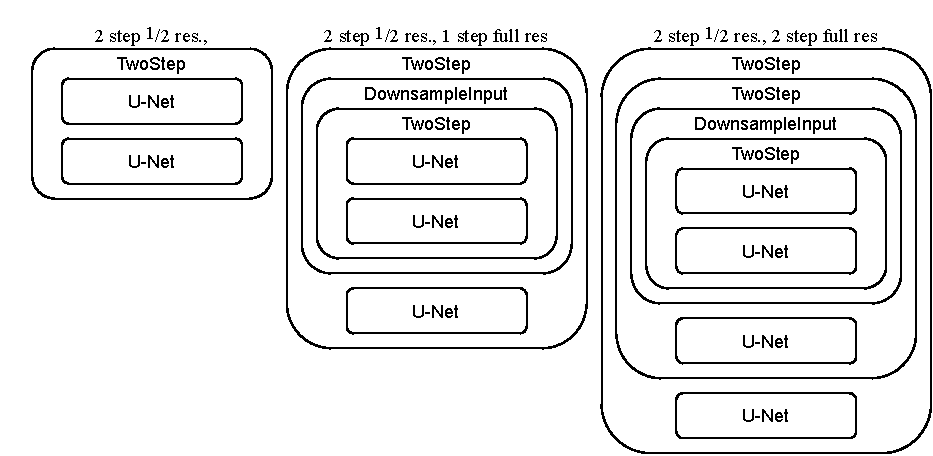
\includegraphics{figs/ICON_OAI-4}\\
    \caption{Architectures used for our OAI results. The low resolution component inside DownsampleInput only requires an 8th the memory and computing power of the whole network, and pretraining it alone makes our overall approach computationally feasible on a single 4 GPU machine. Once it is pretrained, it is plugged into the larger model as shown.}
    \label{fig:oai-arc}
\end{figure}

\subsection{Details}

The ``acceptable number of folds" hyperparameter was set to 200. 200 was the first value tried for this hyperparameter, however this choice was informed by the outcome of previous experiments where $\lambda$ was set manually. 

First, the `low resolution network' is composed of two U-Nets that each take as input a pair of knee images at half resolution, and output a displacement map. These are combined using the operator TwoStep as described above. The low resolution network is trained end to end with $\lambda$ incremented whenever the batch-mean number of folds exceeds 200, as described above. The batch size used is 128, the learning rate is set to $0.00005$, and the network is trained for 16,000 steps. This low resolution pretraining serves to greatly reduce the overall time needed to train the neural network, since much larger batches of images can fit into GPU memory. This step is performed by the included script \path{training_scripts/double_deformable_knee.py}, and the resulting loss curve is reproduced here in Figure 2.

Second, the `low resolution network' is wrapped with a class that downsamples input images, and then combined with a U-Net that takes as input full resolution images, again using the operator TwoStep. The weights of the low resolution network are frozen, and the full resolution network is trained for 75,000 steps, with a learning rate of $0.00005$ and a batch size of 16. This step is performed by the included script \path{training_scripts/hires_finetune_frozen_lowres.py}. The loss curve associated with this step is presented in Figure 2.
Finally, evaluation of the low resolution and full networks is performed using the included notebooks.  \path{DoubleDeformableDICE.ipynb} and \path{DoubleDeformable-HiresDICE.ipynb} respectively. Training was done on a machine with 4 RTX 3090 GPUs, taking 2 days for the low resolution component and 4 days for the high resolution component.
\begin{figure}
    \centering
    Low Resolution Pretraining\par\medskip
    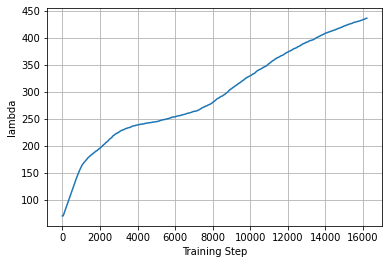
\includegraphics[width=150pt]{OAI-training-curves/low_lambda.png}
    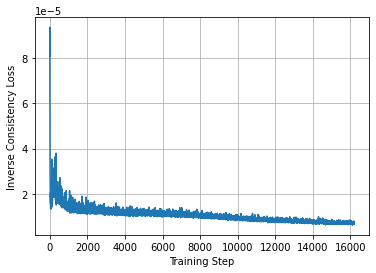
\includegraphics[width=150pt]{OAI-training-curves/low_Linv.png}
    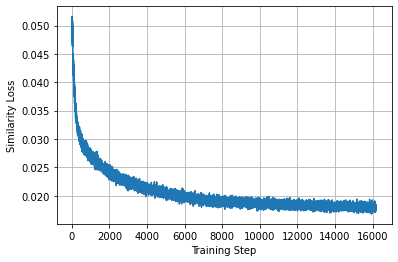
\includegraphics[width=150pt]{OAI-training-curves/low_Lsim.png} \\
    High Resolution Fine Tuning\par\medskip
    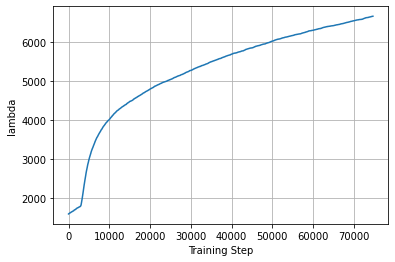
\includegraphics[width=150pt]{OAI-training-curves/high_lambda.png}
    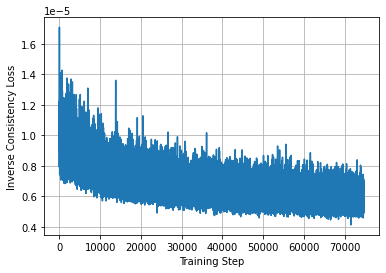
\includegraphics[width=150pt]{OAI-training-curves/high_Linv.png}
    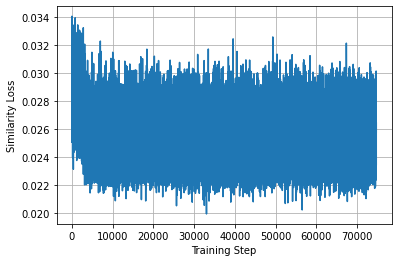
\includegraphics[width=150pt]{OAI-training-curves/high_Lsim.png} \\
    High Resolution Fine Tuning (Second Step)\par\medskip
    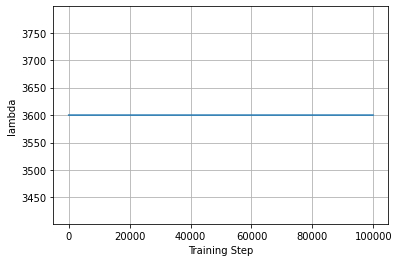
\includegraphics[width=150pt]{OAI-training-curves/high_2_lambda.png}
    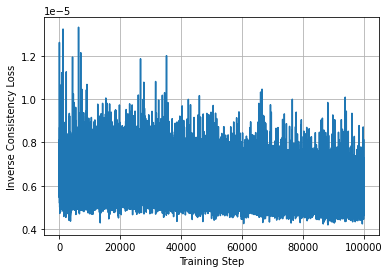
\includegraphics[width=150pt]{OAI-training-curves/high_2_Linv.png}
    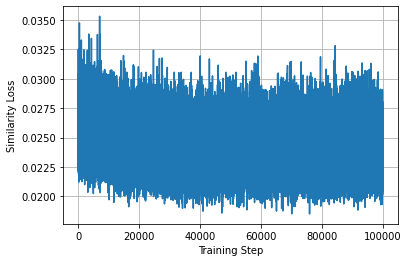
\includegraphics[width=150pt]{OAI-training-curves/high_2_Lsim.png}
    \caption{Training curves for our result on OAI dataset. It is interesting that the required value of $\lambda$ to suppress folding increases over the course of training, and in particular increases rapidly once we begin training in high resolution. Nonetheless, our approach of incrementing $\lambda$ by a fixed amount whenever the number of folds in a batch exceeds a threshold successfully generates smooth transforms.}
    \label{fig:training_curves}
\end{figure}



\opt{for_gig,icml_submission}
{
  \bibliographystyle{icml2021}
  \bibliography{mybibliography}
}
\opt{iccv_submission}
    {
      
      {\small
        \bibliographystyle{ieee_fullname}
        \bibliography{mybibliography}
      }
    }

\end{document}
